\documentclass[english,man]{apa6}

\usepackage{amssymb,amsmath}
\usepackage{ifxetex,ifluatex}
\usepackage{fixltx2e} % provides \textsubscript
\ifnum 0\ifxetex 1\fi\ifluatex 1\fi=0 % if pdftex
  \usepackage[T1]{fontenc}
  \usepackage[utf8]{inputenc}
\else % if luatex or xelatex
  \ifxetex
    \usepackage{mathspec}
    \usepackage{xltxtra,xunicode}
  \else
    \usepackage{fontspec}
  \fi
  \defaultfontfeatures{Mapping=tex-text,Scale=MatchLowercase}
  \newcommand{\euro}{€}
\fi
% use upquote if available, for straight quotes in verbatim environments
\IfFileExists{upquote.sty}{\usepackage{upquote}}{}
% use microtype if available
\IfFileExists{microtype.sty}{\usepackage{microtype}}{}

% Table formatting
\usepackage{longtable, booktabs}
\usepackage{lscape}
% \usepackage[counterclockwise]{rotating}   % Landscape page setup for large tables
\usepackage{multirow}		% Table styling
\usepackage{tabularx}		% Control Column width
\usepackage[flushleft]{threeparttable}	% Allows for three part tables with a specified notes section
\usepackage{threeparttablex}            % Lets threeparttable work with longtable

% Create new environments so endfloat can handle them
% \newenvironment{ltable}
%   {\begin{landscape}\begin{center}\begin{threeparttable}}
%   {\end{threeparttable}\end{center}\end{landscape}}

\newenvironment{lltable}
  {\begin{landscape}\begin{center}\begin{ThreePartTable}}
  {\end{ThreePartTable}\end{center}\end{landscape}}

  \usepackage{ifthen} % Only add declarations when endfloat package is loaded
  \ifthenelse{\equal{\string man}{\string man}}{%
   \DeclareDelayedFloatFlavor{ThreePartTable}{table} % Make endfloat play with longtable
   % \DeclareDelayedFloatFlavor{ltable}{table} % Make endfloat play with lscape
   \DeclareDelayedFloatFlavor{lltable}{table} % Make endfloat play with lscape & longtable
  }{}%



% The following enables adjusting longtable caption width to table width
% Solution found at http://golatex.de/longtable-mit-caption-so-breit-wie-die-tabelle-t15767.html
\makeatletter
\newcommand\LastLTentrywidth{1em}
\newlength\longtablewidth
\setlength{\longtablewidth}{1in}
\newcommand\getlongtablewidth{%
 \begingroup
  \ifcsname LT@\roman{LT@tables}\endcsname
  \global\longtablewidth=0pt
  \renewcommand\LT@entry[2]{\global\advance\longtablewidth by ##2\relax\gdef\LastLTentrywidth{##2}}%
  \@nameuse{LT@\roman{LT@tables}}%
  \fi
\endgroup}


\ifxetex
  \usepackage[setpagesize=false, % page size defined by xetex
              unicode=false, % unicode breaks when used with xetex
              xetex]{hyperref}
\else
  \usepackage[unicode=true]{hyperref}
\fi
\hypersetup{breaklinks=true,
            pdfauthor={},
            pdftitle={Handling missing data in smartphone location logs},
            colorlinks=true,
            citecolor=blue,
            urlcolor=blue,
            linkcolor=black,
            pdfborder={0 0 0}}
\urlstyle{same}  % don't use monospace font for urls

\setlength{\parindent}{0pt}
%\setlength{\parskip}{0pt plus 0pt minus 0pt}

\setlength{\emergencystretch}{3em}  % prevent overfull lines

\ifxetex
  \usepackage{polyglossia}
  \setmainlanguage{}
\else
  \usepackage[english]{babel}
\fi

% Manuscript styling
\captionsetup{font=singlespacing,justification=justified}
\usepackage{csquotes}
\usepackage{upgreek}

 % Line numbering
  \usepackage{lineno}
  \linenumbers


\usepackage{tikz} % Variable definition to generate author note

% fix for \tightlist problem in pandoc 1.14
\providecommand{\tightlist}{%
  \setlength{\itemsep}{0pt}\setlength{\parskip}{0pt}}

% Essential manuscript parts
  \title{Handling missing data in smartphone location logs}

  \shorttitle{Missing Data in Smartphone Location Logs}


  \author{Boaz Sobrado\textsuperscript{1}}

  \def\affdep{{""}}%
  \def\affcity{{""}}%

  \affiliation{
    \vspace{0.5cm}
          \textsuperscript{1} Utrecht University  }

  \authornote{
    \newcounter{author}
    Department of Methodology \& Statistics
    
    Submitted as a research report.

                      Correspondence concerning this article should be addressed to Boaz Sobrado, Postal address. E-mail: \href{mailto:boaz@boazsobrado.com}{\nolinkurl{boaz@boazsobrado.com}}
                }


  \abstract{Using objective location data to infer the mobility measures of
individuals is highly desirable, but methodologically difficult. Using
commercially gathered location logs from smartphones holds great
promise, as they have already been gathered, often span years and can be
associated to individuals. However, due to technical constraints this
data is more sparse and inaccurate than that produced by specialised
equipment. In this paper we present a model which leverages the
periodicity of human mobility in order to impute missing data values.
Moreover, we will assess the performance of the model relative to
currently used methods, such as linear interpolation.}
  \keywords{GPS, Human Mobility \\

    \indent Word count: X
  }





\usepackage{amsthm}
\newtheorem{theorem}{Theorem}
\newtheorem{lemma}{Lemma}
\theoremstyle{definition}
\newtheorem{definition}{Definition}
\newtheorem{corollary}{Corollary}
\newtheorem{proposition}{Proposition}
\theoremstyle{definition}
\newtheorem{example}{Example}
\theoremstyle{definition}
\newtheorem{exercise}{Exercise}
\theoremstyle{remark}
\newtheorem*{remark}{Remark}
\newtheorem*{solution}{Solution}
\begin{document}

\maketitle

\setcounter{secnumdepth}{0}



How active people are and how they interact with their environment
affects a wide range of outcomes including health, income and social
capital (Goodchild \& Janelle, 2010). A better understanding of both
within-person and between-person variability in geospatial patterns
could be conducive to better social, health and urban-planning policies.
Yet a large part of studies on human mobility are largely based on
pen-and-paper travel diaries. These surveys have known methodological
flaws, such as the short period of data collection (due to costs and
burden to respondents), the underreporting of short trips (Wolf,
Oliveira, \& Thompson, 2003) and the underestimation of the duration of
commutes (Delclòs-Alió, Marquet, \& Miralles-Guasch, 2017).

These obstacles can be overcome by using objective data on human
mobility. The Global Positioning System (GPS), which uses the distance
between a device and a number of satellites to determine location,
provides such data. Within behavioural science, this type of data has
been used to investigate topics such as the effects of the food
environment on eating patterns (Zenk, Schulz, \& Odoms-Young, 2009), the
movement correlates of personality (G. M. Harari et al., 2016), academic
performance (Wang, Harari, Hao, Zhou, \& Campbell, 2015) and bipolar
disorder (Palmius et al., 2017).

In most of these studies participants are given a specialised device,
resulting in accurate mobility GPS data (\emph{specialised logs}).
However, Barnett and Onnela (2016) point out that these studies are not
scalable due to cost and burden to participants. Moreover, they may be
biased because of the introduction of a new device to the participant's
life. Because of these drawbacks, specialised logs usually span a short
amount of time. Barnett and Onnela (2016) advocate installing a
custom-made tracking app on user's phones (\emph{custom logs}). Another
solution is to take advantage of existing smartphone location logs, such
as Google Location History, which store location information of millions
of users spanning several years (Location History, 2017)
(\emph{secondary logs}). By law, logs can be accessed and shared by
users for free (Commission, 2017). Yet, because they were created for
non-academic purposes under engineering constraints, the sensors do not
monitor continuously and the resulting logs can be sparse and
inaccurate. Hence, two important challenges are dealing with measurement
noise and missing data.

Missing data is a pervasive issue as it can arise due to multiple
reasons. Technical reasons include signal loss, battery failure and
device failure. Behavioural reasons include leaving the phone at home,
switching the phone off, switching location measurements off, and so on.
As a result, applied researchers are often left with wide temporal gaps
with no measurements. For instance, different groups studying the effect
of bipolar disorder on human movement have reported missing data rates
between 30\% to 50\% (Grünerbl et al., 2015; Palmius et al., 2017; Saeb
et al., 2015). Similar trends are consistently reported in other fields
(e.g. G. M. Harari et al., 2016; Jankowska, Schipperijn, \& Kerr, 2015).

There is currently no golden standard in how to deal with missing data
in custom or secondary logs (Barnett \& Onnela, 2016). Traditional
missing data methods, such as mean imputation, cannot be used easily in
spatiotemporal data because the measurements are correlated in time and
space. For example, assume the simplistic case that an individual spends
almost half her time at work, half her time at home and a small amount
of time commuting between the two along a angled path. Using mean
imputation would result in imputed values of her being at the geometric
midpoint between the home and work for all missing values, even though
she has never been there and never will be. Worringly, Jankowska et al.
(2015) have pointed out that there is often little transparency
regarding decisions of how to deal with missing data.

The accuracy of GPS measurements in smartphones is substantially lower
than in professional grade GPS trackers. For example, Android phones
collect location information through a variety of methods, such as from
WiFi access points, cellphone triangulation, and GPS measurements. They
use different methods due to computational and battery constraints (M.
Y. Chen et al., 2006; LaMarca et al., 2005).In professional grade GPS
trackers less than 80\% of measurements fall within 10 meters of the
true location. GPS measures are reported to be most inaccurate in high
density urban locations and indoors (S. Duncan et al., 2013; Schipperijn
et al., 2014). Unfortunately for social scientists, this happens to be
where most people in the developed world tend to spend most of their
time.

On the other hand, noisy data can lead to inaccurate conclusions if it
is not accounted for, such as overestimating the movement of
individuals. For instance, suppose that a naive researcher calculates
the distance travelled by an individual by drawing a line between each
measured point and calculating the sum of the length of all of these
lines. If there is noise, the measurements will vary even though the
individual is not moving. If the measurements are frequent, then the
researcher will end up with a lot of movement, even though the
individual did not move at all. The problem is further complicated by
the fact that missing data and noisy measurements are related to each
other. For instance, methods used by researchers to reduce noise, such
as throwing out inaccurate measurements (e.g. Palmius et al., 2017) can
exacerbate the severity of the missing data problem.

In this paper we will compare methods used to deal with measurement
error and missing data in mobility patterns from secondary GPS logs.

\section{A concrete example}\label{a-concrete-example}

Given that there is little literature on dealing with missing data in
custom or secondary logs it is worth illustrating the typical
characteristics of this data using an example data set. The example
dataset comes from the Google Location History of a single individual
and spans from January 2013 to January 2017. It was recorded with
multiple different Android devices and contains 814 941 measurements,
with approximately 742 measurements per day
(\(\widehat{\sigma}\)=868.15). The dataset contains a wide range of
variables including inferred activity and velocity. For the purposes of
this paper we will focus only on latitude, longitude, accuracy (defined
below) and a timestamp.

\subsection{Location logs and
notation}\label{location-logs-and-notation}

GPS measurements report our location on a three dimensional planet, yet
we are interested in placing these measurements on a two dimensional
map. Projecting three dimensional measurements onto a two dimensional
plane results in errors, in order to minimise these errors we borrow an
error minimising projection method from Barnett and Onnela (2016).

Let a persons' true location on this two-dimensional plane be
\(G(t) = [G_x(t) G_y(t)]\) where \(G_x(t)\) and \(G_y(t)\) denote the
location of the individual at time \(t\) on the x-axis and y-axis
respectively. Moreover, let \(D \in \mathbb{R}^2\) be the recorded data
containing lattitude and longitude. In addition, let \(a\) denote the
estimated accuracy of the recorded data. accuracy. \(G(t)\), \(D\) and
\(a\) are indexed by time labled by the set \(T = t_1 < ... < t_{n+1}\).
For simplicity, let each entry in the discrete index set \(T\) represent
a 5 minute window. The measure of accuracy \(a_t\) is given in meters
such that it represents the radius of a 67\% confidence circle. If
\(D_t = \emptyset\) it is considered \emph{missing} and it is not
missing otherwise.

\subsubsection{Accuracy in location
logs}\label{accuracy-in-location-logs}

In the example data set the distribution of \(a\) is highly right
skewed, with a median of 28, \(\mu = 127\) and the maximum value at 26
km. Palmius et al. (2017) note that in their Android based custom logs
inaccurate location values are interspersed between more accurate
location values at higher sample rates per hour. We observe similar
patterns in secondary logs. Figure 1 shows how accuracy tends to vary as
a function of user behaviour, time and location. There are several
recurring low-accuracy points, most likely cell-phone triangulation
towers.

\begin{figure}
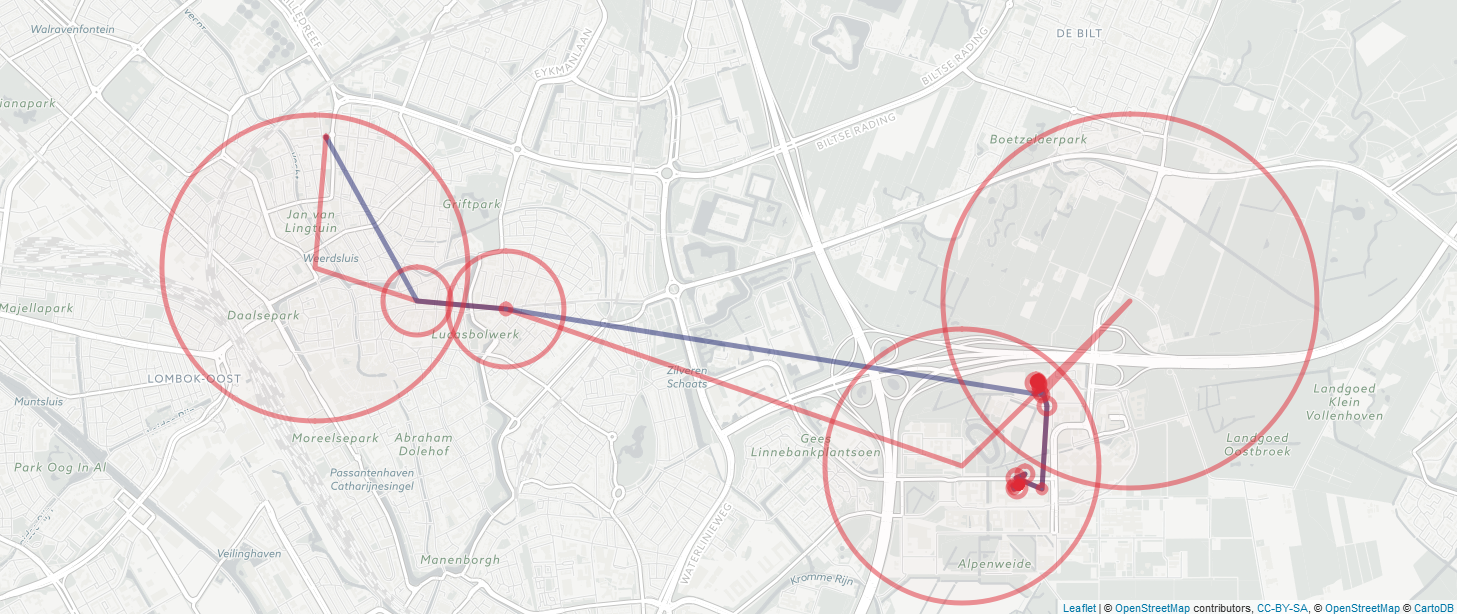
\includegraphics[width=1\linewidth]{img/journeyTillMiddayBoaz} \caption{Measurement accuracy of each logged measurement in a morning journey. The red circles denote the accuracy of all logged measurement points (the raw data). The points connected in time are connected by a line. The blue line shows the path without the most inaccurate (accuracy > 400 meters) points filtered out. The red line shows the path with all measurements included. }\label{fig:accuracyPlot}
\end{figure}

\begin{figure}
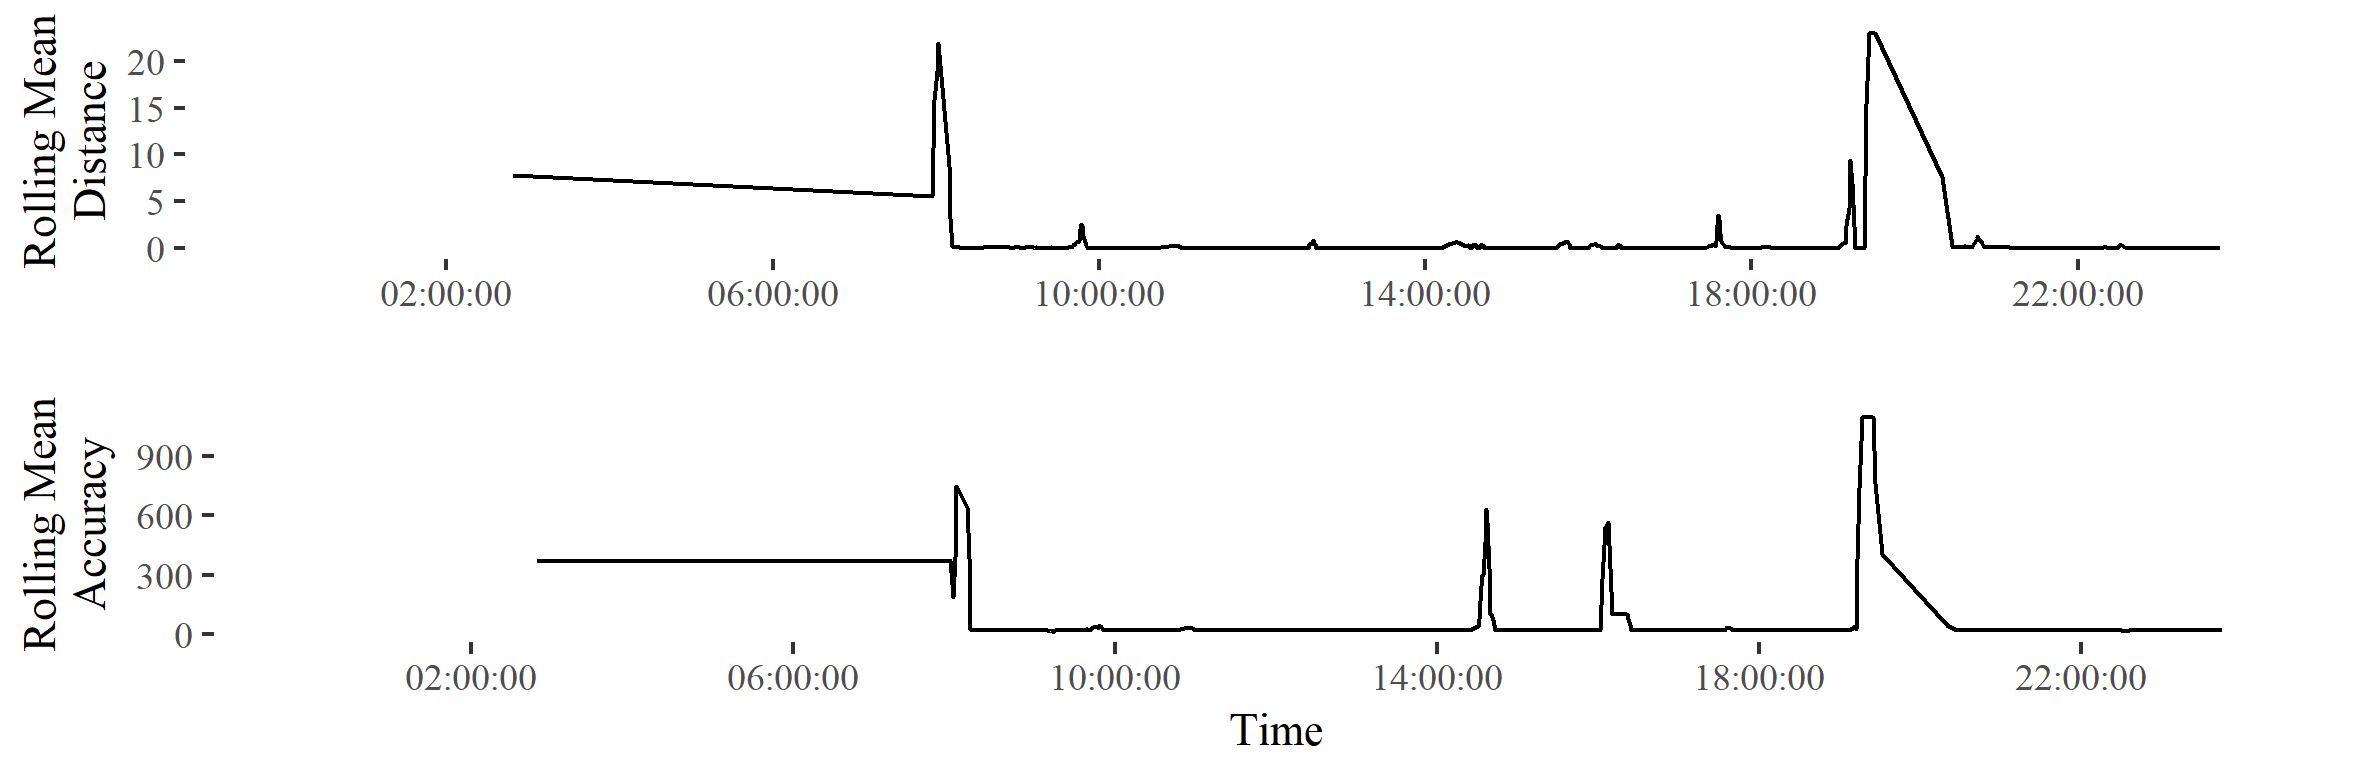
\includegraphics[width=1\linewidth]{img/accuracyLocShift} \caption{The accuracy of raw measures with time on the x-axis and accuracy on the y-axis. The colour scale shows the distance between the measurement and the previous point.}\label{fig:accuracyPlot2}
\end{figure}

\subsubsection{Missingness}\label{missingness}

Over 54\% of the data is missing for the entire duration of the log.
However,this is misleading as there are several long periods with no
measurements whatsoever. The structure of missingness of a day with
measurements is shown below.

\begin{figure}
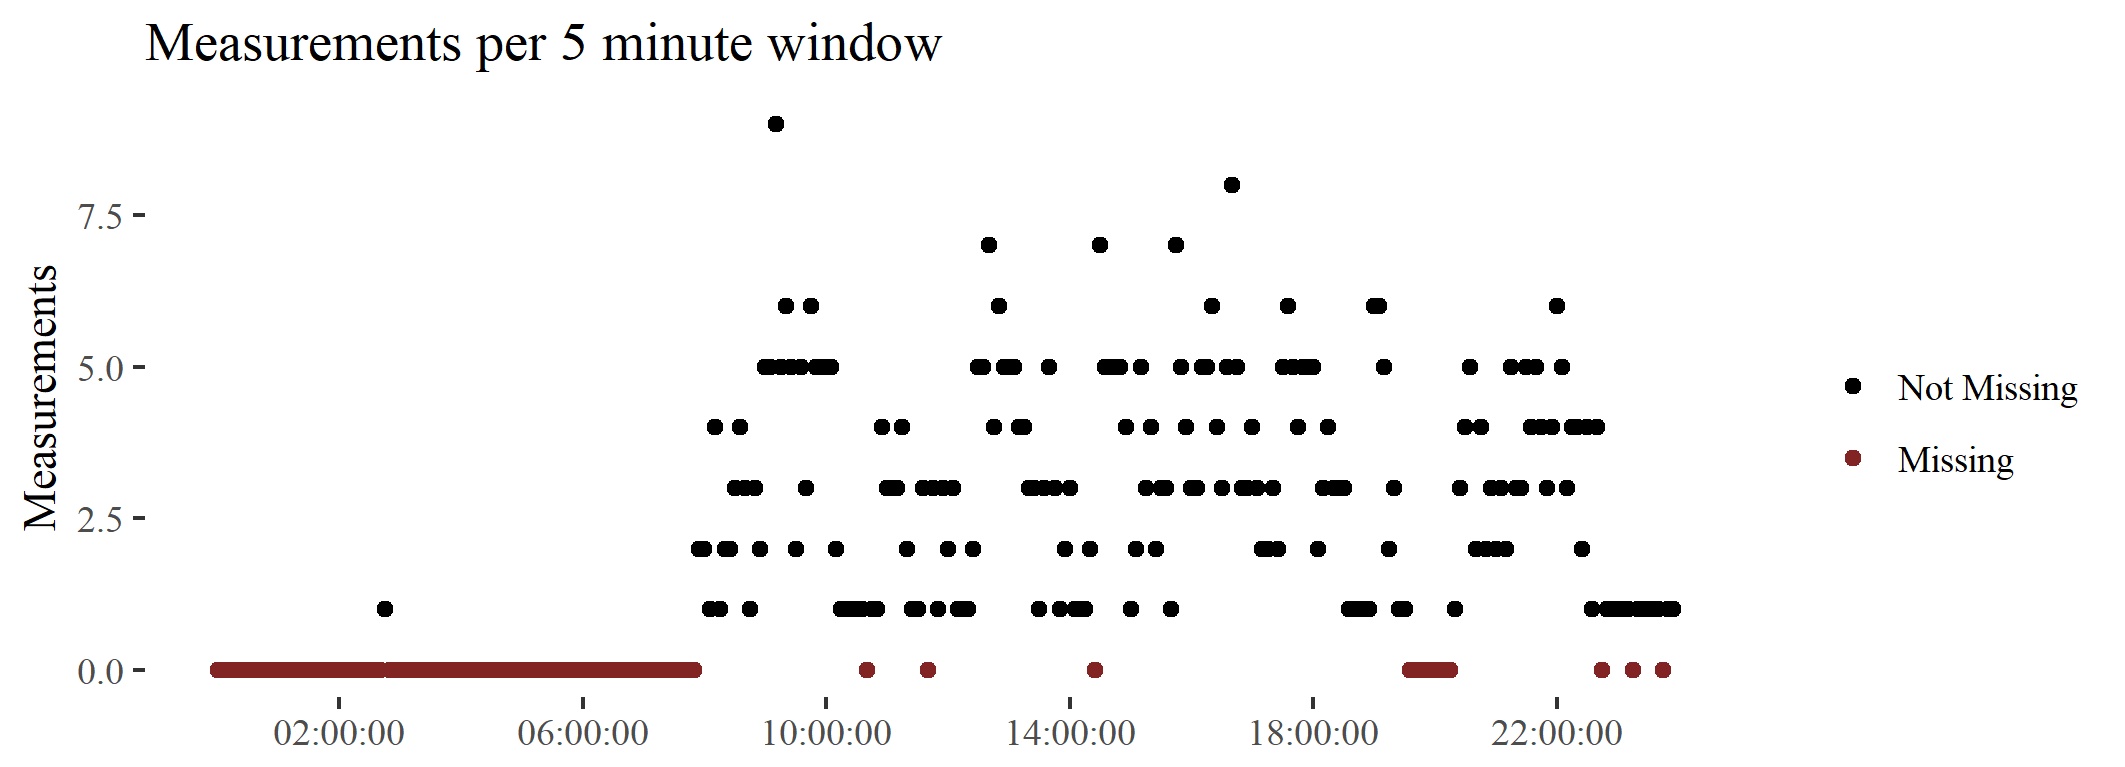
\includegraphics[width=1\linewidth]{img/missingBoaz5minExample} \caption{Example of missing data over a day. The x-axis denotes time, the y-axis shows how many measurements are made and each point is a five minute window. For this day there were several periods with no information. These points are filled with red and lie on the x-axis.}\label{fig:measurementsPerDay}
\end{figure}

\subsection{Current methods for imputing missing spatiotemporal
data}\label{current-methods-for-imputing-missing-spatiotemporal-data}

As we have mentioned before, Jankowska et al. (2015) point out that
there is little transparency regarding decisions of how to deal with
missing data in GPS mobility logs. We suspect this is because the highly
interdisciplinary nature of the problem means researchers are unaware of
potential solutions. For this reason, we consider it important to
briefly discuss a few methods one could consider in order to deal with
measurement inaccuracy and missing data problems in spatiotemporal data.
In doing so, we will argue that state space models (SSMs) and
spatiotemporal imputation methods, which are extensively used to model
missing and noisy spatiotemporal data, are not well suited to deal with
human mobility patterns. Moreover, we discuss in detail two approaches
by Palmius et al. (2017) and Barnett and Onnela (2016) which deal
explicitly with missing data in mobility patterns from smartphone GPS
logs.

There is a vast literature of using SSMs to improve measurements
accuracy and deal with missing data. Behavioural ecologists for
instance, have used SSMs extensively to explain how animals interact
with their environment (Patterson, Thomas, Wilcox, Ovaskainen, \&
Matthiopoulos, 2008). These models can be quite complex, for example
Preisler, Ager, Johnson, and Kie (2004) uses Markovian movement
processes to characterise the effect of roads, food patches and streams
on cyclical elk movements. The most well studied SSM is the Kalman
filter, which is the optimal algorithm for inferring linear Gaussian
systems. In fact, the extended Kalman filter is the de facto standard
for GPS navigation (Z. Chen \& Brown, 2013). The advantage of state
space models is that they are flexible, deal with measurement
inaccuracy, include information from different sources and can be used
in real time.

However, the main limitation of SSMs is that they ignore the fact that
humans have regular movement routines, such as going to work or shopping
for groceries on weekends. This limitation is due to the fact that SSMs
are based on the Markov property. Thus, the estimated location \(G(t)\)
at timepoint \(t\) is often based only upon measurements \(D_t\),
\(D_{t-1}\) and ignores all \(D_{t-i}|i\geq2\). Hierarchical structuring
and conditioning on a larger context have been suggested as ways to
improve the performance of Markovian models, but these solutions are
often computationally intractable or unfeasible (Sadilek \& Krumm,
2016). For this reason we do not consider SSMs to be useful for imputing
missing data, although they could be of use in filtering noise.

In addition to SSMs there are spatiotemporal imputation methods often
used in climate or geological research for estimating missing data. For
instance, Feng, Nowak, O'Neill, and Welsh (2014) illustrate their CUTOFF
method, which relies on estimating missing values using the nearest
observed neighbours in time, using rainfall data from dozens of gauging
stations across Australia. Similarly, Z. Zhang et al. (2017) use a
variety of machine learning methods to present their model based on
underground water data in China.

The difficulty of applying this class of spatiotemporal imputation
models to human mobility tracks lies in the fact that these models
generally assume fixed measurement stations (such as rainfall gauging
stations). While Feng et al. (2014) claim their model could be used to
establish mobility patterns, ostensibly by dividing the sample space
into rasters analogous to measurement stations indicating a probability
of the individual being there, this seems to be computationally
unfeasible. To our knowledge such models have not been implemented for
mobility traces.

On the other hand, a few researchers have explicitly attempted to impute
missing data from human mobility patterns. Palmius et al. (2017) deal
with the measuremement inaccuracy of \(D\) in custom logs by removing
from the data set all unique low-accuracy \(a\) data points that had
\(\frac{d}{dt}D > 100 \frac{km}{h}\). Subsequently the researchers down
sample the data to a sample rate of 12 per hour using a median filter.
Moreover, Palmius et al. (2017) explain:

\begin{quote}
\enquote{If the standard deviation of {[}\(D\){]} in both latitude and
longitude within a 1 h epoch was less than 0.01 km, then all samples
within the hour were set to the mean value of the recorded data,
otherwise a 5 min median filter window was applied to the recorded
latitude and longitude in the epoch}.
\end{quote}

Missing data was imputed using the mean of measurements close in time if
the participant was recorded within 500m of either end of a missing
section and the missing section had a length of \(\leq 2h\) or
\(\leq 12h\) after 9pm.

Barnett and Onnela (2016) follow a different approach which is, to the
best of our knowledge, the only pricipled approach to dealing with
missing data in human mobility data. Barnett and Onnela (2016) work with
custom logs where location is measured for 2 minutes and subsequently
not measured for 10 minutes. In the words of the authors, Barnett and
Onnela (2016) handle missing data by:

\begin{quote}
\enquote{simulat{[}ing{]} flights and pauses over the period of
missingness where the direction, duration, and spatial length of each
flight, the fraction of flights versus the fraction of pauses, and the
duration of pauses are sampled from observed data.}
\end{quote}

This method can be extended to imputing the data based on temporally,
spatially or periodically close flights and pauses. In other words, for
a given missing period, the individual's mobility can be estimated based
on measured movements in that area, at that point in time or movements
in the last 24 hours (\emph{circadian proximity}).

\subsection{Methods}\label{methods}

\subsubsection{Datasets \& Analyses}\label{datasets-analyses}

The data used to train the imputation methods was collected between 2013
and 2017 on different Android devices from several individuals (table
1).

\begin{table}

\caption{\label{tab:datadetailsTable}Table with descriptives about the data sets used to build the imputation methods. }
\centering
\begin{tabular}[t]{l|r|r|r|r|r}
\hline
Log duration & Logged days & Observations & Missing days & Missing data & Mean Accuracy\\
\hline
From 2013-02-06 to 2017-03-29 & 1512 & 646376 & 635 & 0.22 & 127.78\\
\hline
From 2016-07-14 to 2017-05-10 & 300 & 158382 & 3 & 0.41 & 1394.60\\
\hline
From 2014-01-22 to 2017-01-23 & 1097 & 814941 & 80 & 0.25 & 121.83\\
\hline
\end{tabular}
\end{table}

In addition to the secondary logs, participants also volunteered to
carry with them a specialised GPS tracker for a week. This specialised
log was used to evaluate the models.

Analyses were performed using R and a multitude of other statistical
packages ({\textbf{???}}; Bivand, Pebesma, \& Gomez-Rubio, 2013; E. J.
Pebesma \& Bivand, 2005; R Core Team, 2017; Wickham, 2009; Wickham \&
Francois, 2016).

\subsubsection{Data pre-processing \&
filtering}\label{data-pre-processing-filtering}

The goal of filtering was to remove noise from the measurements and to
aggregate multiple measurements into 12 per hour. Three different
filtering methods were tested:

\begin{enumerate}
\def\labelenumi{\arabic{enumi}.}
\tightlist
\item
  The filtered rolling-median downsampling method described by Palmius
  et al. (2017).
\item
  A weighted mean approach taking \(f(a)\) as a weight.
\item
  A Kalman filter commonly used for GPS measurements (Doust, 2013).
\end{enumerate}

The output of all of these methods was taken as the input of the
imputation methods.

\subsubsection{Imputation methods}\label{imputation-methods}

Three imputation methods were selected in order to cover a wide range of
techniques applied in the literature:

\begin{enumerate}
\def\labelenumi{\arabic{enumi}.}
\tightlist
\item
  Mean imputation as described by Palmius et al. (2017).
\item
  The model developed by Barnett and Onnela (2016) using spatial,
  temporal and circadian proximity.
\item
  Simple linear interpolation was used as a benchmark model.
\end{enumerate}

\subsubsection{Evaluation criteria}\label{evaluation-criteria}

The entire length of the secondary logs were used as a training set. The
specialised logs were used as a test set. The missing data imputation
models were evaluated both directly, and on two computed measures:
amount of trips made and distance traveled.

The direct evaluation involved calculating the error of each \(D_t\)
compared to \(G(t)\) approximated by the specialised log. The error
measures used were root mean square error (RMSE) and mean absolute error
(MAE).

The evaluation on computed measures involved calculating a mobility
trace following the rectangular method of Rhee, Shin, Hong, Lee, and
Chong (2007) for each imputed dataset. Like Barnett and Onnela (2016) we
calculate bias by substracting the estimated measure under each approach
for the same measure calculated on the full data. For simulation-based
imputation approaches a mean value over 100 samples was taken.

\newpage

\section{References}\label{references}

\setlength{\parindent}{-0.5in} \setlength{\leftskip}{0.5in}

\hypertarget{refs}{}
\hypertarget{ref-barnett_inferring_2016}{}
Barnett, I., \& Onnela, J.-P. (2016). Inferring Mobility Measures from
GPS Traces with Missing Data. \emph{arXiv:1606.06328 {[}Stat{]}}.
Retrieved from \url{http://arxiv.org/abs/1606.06328}

\hypertarget{ref-sp2}{}
Bivand, R. S., Pebesma, E., \& Gomez-Rubio, V. (2013). \emph{Applied
spatial data analysis with R, second edition}. Springer, NY. Retrieved
from \url{http://www.asdar-book.org/}

\hypertarget{ref-chen_practical_2006}{}
Chen, M. Y., Sohn, T., Chmelev, D., Haehnel, D., Hightower, J., Hughes,
J., \ldots{} Varshavsky, A. (2006). Practical Metropolitan-Scale
Positioning for GSM Phones. In \emph{UbiComp 2006: Ubiquitous Computing}
(pp. 225--242). Springer, Berlin, Heidelberg.
doi:\href{https://doi.org/10.1007/11853565_14}{10.1007/11853565\_14}

\hypertarget{ref-chen_state_2013}{}
Chen, Z., \& Brown, E. N. (2013). State space model.
\emph{Scholarpedia}, \emph{8}(3), 30868.
doi:\href{https://doi.org/10.4249/scholarpedia.30868}{10.4249/scholarpedia.30868}

\hypertarget{ref-commission_protecting_2017}{}
Commission, E. (2017). Protecting your data: Your rights - European
Commission. Retrieved from
\url{http://ec.europa.eu/justice/data-protection/individuals/rights/index_en.htm}

\hypertarget{ref-delclos-alio_keeping_2017}{}
Delclòs-Alió, X., Marquet, O., \& Miralles-Guasch, C. (2017). Keeping
track of time: A Smartphone-based analysis of travel time perception in
a suburban environment. \emph{Travel Behaviour and Society},
\emph{9}(Supplement C), 1--9.
doi:\href{https://doi.org/10.1016/j.tbs.2017.07.001}{10.1016/j.tbs.2017.07.001}

\hypertarget{ref-doust_smoothing_2013}{}
Doust, P. (2013). \emph{Smoothing - Smooth GPS data - Stack Overflow}.
Retrieved from
\url{https://stackoverflow.com/questions/1134579/smooth-gps-data}

\hypertarget{ref-duncan_portable_2013}{}
Duncan, S., Stewart, T. I., Oliver, M., Mavoa, S., MacRae, D., Badland,
H. M., \& Duncan, M. J. (2013). Portable global positioning system
receivers: Static validity and environmental conditions. \emph{American
Journal of Preventive Medicine}, \emph{44}(2), e19--29.
doi:\href{https://doi.org/10.1016/j.amepre.2012.10.013}{10.1016/j.amepre.2012.10.013}

\hypertarget{ref-feng_cutoff:_2014}{}
Feng, L., Nowak, G., O'Neill, T., \& Welsh, A. (2014). CUTOFF: A
spatio-temporal imputation method. \emph{Journal of Hydrology},
\emph{519}, 3591--3605.
doi:\href{https://doi.org/10.1016/j.jhydrol.2014.11.012}{10.1016/j.jhydrol.2014.11.012}

\hypertarget{ref-goodchild_toward_2010}{}
Goodchild, M. F., \& Janelle, D. G. (2010). Toward critical spatial
thinking in the social sciences and humanities. \emph{GeoJournal},
\emph{75}(1), 3--13.
doi:\href{https://doi.org/10.1007/s10708-010-9340-3}{10.1007/s10708-010-9340-3}

\hypertarget{ref-grunerbl_smartphone-based_2015}{}
Grünerbl, A., Muaremi, A., Osmani, V., Bahle, G., Ohler, S., Tröster,
G., \ldots{} Lukowicz, P. (2015). Smartphone-based recognition of states
and state changes in bipolar disorder patients. \emph{IEEE Journal of
Biomedical and Health Informatics}, \emph{19}(1), 140--148.
doi:\href{https://doi.org/10.1109/JBHI.2014.2343154}{10.1109/JBHI.2014.2343154}

\hypertarget{ref-harari_using_2016}{}
Harari, G. M., Lane, N. D., Wang, R., Crosier, B. S., Campbell, A. T.,
\& Gosling, S. D. (2016). Using Smartphones to Collect Behavioral Data
in Psychological Science: Opportunities, Practical Considerations, and
Challenges. \emph{Perspectives on Psychological Science}, \emph{11}(6),
838--854.
doi:\href{https://doi.org/10.1177/1745691616650285}{10.1177/1745691616650285}

\hypertarget{ref-jankowska_framework_2015}{}
Jankowska, M. M., Schipperijn, J., \& Kerr, J. (2015). A Framework For
Using GPS Data In Physical Activity And Sedentary Behavior Studies.
\emph{Exercise and Sport Sciences Reviews}, \emph{43}(1), 48--56.
doi:\href{https://doi.org/10.1249/JES.0000000000000035}{10.1249/JES.0000000000000035}

\hypertarget{ref-lamarca_place_2005}{}
LaMarca, A., Chawathe, Y., Consolvo, S., Hightower, J., Smith, I.,
Scott, J., \ldots{} Schilit, B. (2005). Place Lab: Device Positioning
Using Radio Beacons in the Wild. In \emph{Pervasive Computing} (pp.
116--133). Springer, Berlin, Heidelberg.
doi:\href{https://doi.org/10.1007/11428572_8}{10.1007/11428572\_8}

\hypertarget{ref-location_history_timeline_2017}{}
Location History, G. (2017). Timeline. Retrieved from
\url{https://www.google.com/maps/timeline?pb}

\hypertarget{ref-palmius_detecting_2017}{}
Palmius, N., Tsanas, A., Saunders, K. E. A., Bilderbeck, A. C., Geddes,
J. R., Goodwin, G. M., \& Vos, M. D. (2017). Detecting Bipolar
Depression From Geographic Location Data. \emph{IEEE Transactions on
Biomedical Engineering}, \emph{64}(8), 1761--1771.
doi:\href{https://doi.org/10.1109/TBME.2016.2611862}{10.1109/TBME.2016.2611862}

\hypertarget{ref-patterson_statespace_2008}{}
Patterson, T. A., Thomas, L., Wilcox, C., Ovaskainen, O., \&
Matthiopoulos, J. (2008). State--space models of individual animal
movement. \emph{Trends in Ecology \& Evolution}, \emph{23}(2), 87--94.
doi:\href{https://doi.org/10.1016/j.tree.2007.10.009}{10.1016/j.tree.2007.10.009}

\hypertarget{ref-sp1}{}
Pebesma, E. J., \& Bivand, R. S. (2005). Classes and methods for spatial
data in R. \emph{R News}, \emph{5}(2), 9--13. Retrieved from
\url{https://CRAN.R-project.org/doc/Rnews/}

\hypertarget{ref-preisler_modeling_2004}{}
Preisler, H. K., Ager, A. A., Johnson, B. K., \& Kie, J. G. (2004).
Modeling animal movements using stochastic differential equations.
\emph{Environmetrics 15: P. 643-657}. Retrieved from
\url{https://www.fs.usda.gov/treesearch/pubs/33038}

\hypertarget{ref-base}{}
R Core Team. (2017). \emph{R: A language and environment for statistical
computing}. Vienna, Austria: R Foundation for Statistical Computing.
Retrieved from \url{https://www.R-project.org/}

\hypertarget{ref-rhee_human_2007}{}
Rhee, I., Shin, M., Hong, S., Lee, K., \& Chong, S. (2007). Human
Mobility Patterns and Their Impact on Routing in Human-Driven Mobile
Networks. \emph{ACM HotNets 2007}. Retrieved from
\url{http://koasas.kaist.ac.kr/handle/10203/160927}

\hypertarget{ref-sadilek_far_2016}{}
Sadilek, A., \& Krumm, J. (2016). Far Out: Predicting Long-Term Human
Mobility. \emph{Microsoft Research}. Retrieved from
\url{https://www.microsoft.com/en-us/research/publication/far-predicting-long-term-human-mobility/}

\hypertarget{ref-saeb_mobile_2015}{}
Saeb, S., Zhang, M., Karr, C. J., Schueller, S. M., Corden, M. E.,
Kording, K. P., \& Mohr, D. C. (2015). Mobile Phone Sensor Correlates of
Depressive Symptom Severity in Daily-Life Behavior: An Exploratory
Study. \emph{Journal of Medical Internet Research}, \emph{17}(7), e175.
doi:\href{https://doi.org/10.2196/jmir.4273}{10.2196/jmir.4273}

\hypertarget{ref-schipperijn_dynamic_2014}{}
Schipperijn, J., Kerr, J., Duncan, S., Madsen, T., Klinker, C. D., \&
Troelsen, J. (2014). Dynamic Accuracy of GPS Receivers for Use in Health
Research: A Novel Method to Assess GPS Accuracy in Real-World Settings.
\emph{Frontiers in Public Health}, \emph{2}, 21.
doi:\href{https://doi.org/10.3389/fpubh.2014.00021}{10.3389/fpubh.2014.00021}

\hypertarget{ref-wang_smartgpa:_2015}{}
Wang, R., Harari, G., Hao, P., Zhou, X., \& Campbell, A. T. (2015).
SmartGPA: How Smartphones Can Assess and Predict Academic Performance of
College Students. In \emph{Proceedings of the 2015 ACM International
Joint Conference on Pervasive and Ubiquitous Computing} (pp. 295--306).
New York, NY, USA: ACM.
doi:\href{https://doi.org/10.1145/2750858.2804251}{10.1145/2750858.2804251}

\hypertarget{ref-ggplot2}{}
Wickham, H. (2009). \emph{Ggplot2: Elegant graphics for data analysis}.
Springer-Verlag New York. Retrieved from \url{http://ggplot2.org}

\hypertarget{ref-dplyr}{}
Wickham, H., \& Francois, R. (2016). \emph{Dplyr: A grammar of data
manipulation}. Retrieved from
\url{https://CRAN.R-project.org/package=dplyr}

\hypertarget{ref-wolf_impact_2003}{}
Wolf, J., Oliveira, M., \& Thompson, M. (2003). Impact of Underreporting
on Mileage and Travel Time Estimates: Results from Global Positioning
System-Enhanced Household Travel Survey. \emph{Transportation Research
Record: Journal of the Transportation Research Board}, \emph{1854},
189--198. doi:\href{https://doi.org/10.3141/1854-21}{10.3141/1854-21}

\hypertarget{ref-zenk_how_2009}{}
Zenk, S. N., Schulz, A. J., \& Odoms-Young, A. (2009). How Neighborhood
Environments Contribute to Obesity. \emph{The American Journal of
Nursing}, \emph{109}(7), 61--64.
doi:\href{https://doi.org/10.1097/01.NAJ.0000357175.86507.c8}{10.1097/01.NAJ.0000357175.86507.c8}

\hypertarget{ref-zhang_application_2017}{}
Zhang, Z., Yang, X., Li, H., Li, W., Yan, H., \& Shi, F. (2017).
Application of a novel hybrid method for spatiotemporal data imputation:
A case study of the Minqin County groundwater level. \emph{Journal of
Hydrology}, \emph{553}(Supplement C), 384--397.
doi:\href{https://doi.org/10.1016/j.jhydrol.2017.07.053}{10.1016/j.jhydrol.2017.07.053}






\end{document}
